\documentclass{book}

\usepackage{gensymb}
\usepackage{graphicx}
\usepackage[hidelinks]{hyperref}
\hypersetup{
	linktoc=all
}
\usepackage{siunitx}
\usepackage{textgreek}

\begin{document}
\title{Vitamins}
\author{Radu-Mihai Rotariu}
\maketitle
\pagenumbering{roman}
\tableofcontents\newpage
\pagenumbering{arabic}

\chapter{Vitamin A}
\begin{figure}[h]
	\caption{Chemical structure of retinol}
	\centering 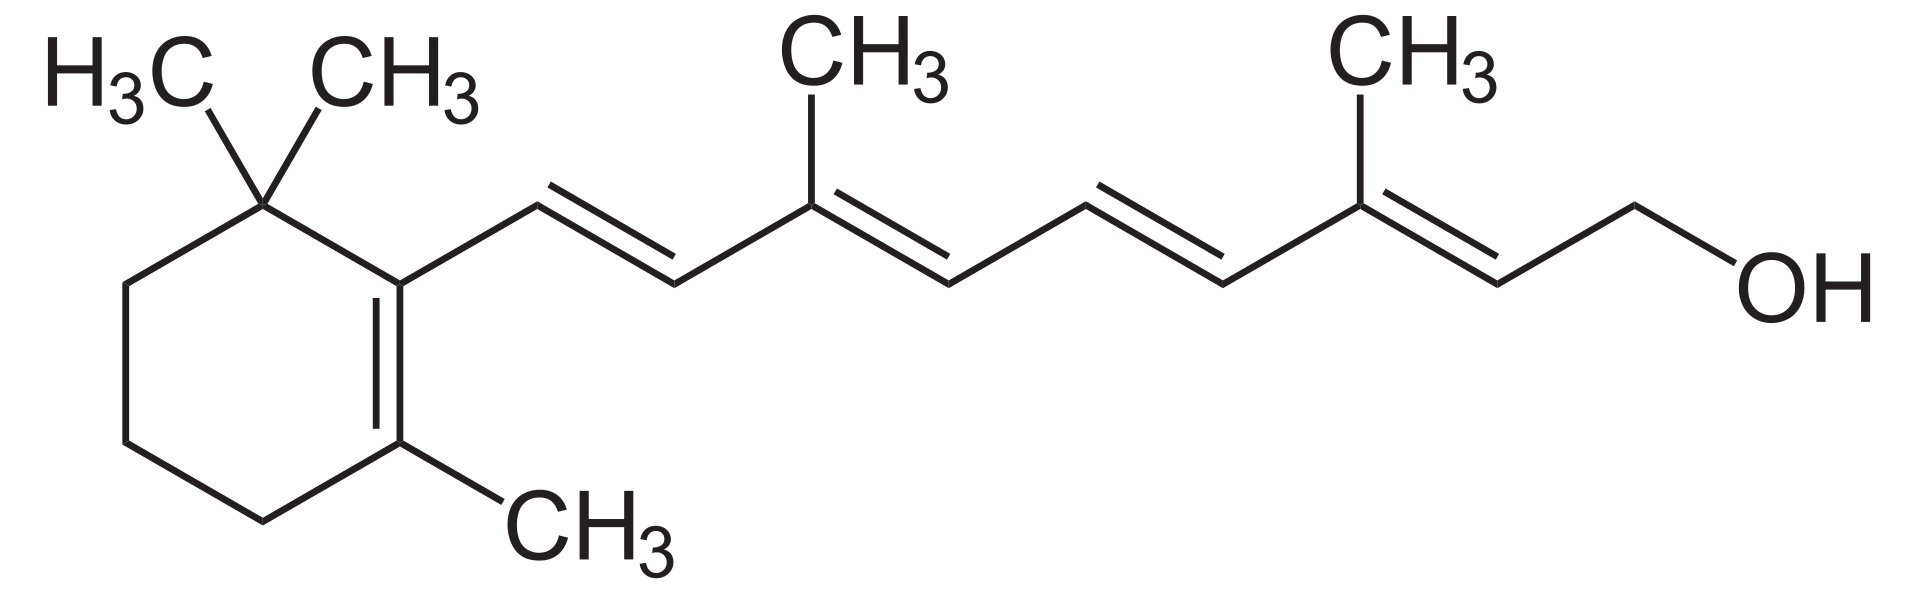
\includegraphics[width=\textwidth]{images/Vitamin_A_chemical_structure}
\end{figure}
\newpage

\section{About}
Vitamin A is a fat-soluble vitamin and essential nutrient. The term itself refers to a family of compounds, which includes: retinol, retinal (also known as retinaldehyde), retinoic acid, and provitamin carotenoids (precursors), most notable being \textbeta-carotene.

Vitamin A is found in food in two forms:
\begin{itemize}
	\item Retinol, found in animal-sourced foods, either as retinol or bound to a fatty acid to become a retinyl ester.
	\item Carotenoids \textalpha-carotene, \textbeta-carotene, \textgamma-carotene, and the xanthophyll \textbeta-cryptoxanthin. All of these carotenoids function as precursors to vitamin A in herbivores and omnivores which possess the required cleaving enzymes needed to convert the carotenoids to retinal and then the retinal to retinol. Some carnivore animals lack this enzyme. All the other carotenoids have no vitamin activity.
\end{itemize}

\section{Measurement unit}
The agreed upon standard measurement unit is 1\textmu g, which is $\sim$0.33 nmol of retinol. It's also referred to as a \textmu g RAE (Retinol Activity Equivalent).

Since four of the carotenoids can be converted into retinol, an equivalency has been established between the standard measurement unit for retinol and each of the precursors.

As such, here is a list of the standard units of measurements for retinol and its equivalent for all the precursors:

\begin{table}[h]
	\caption{VItamin A standard measurement units}
	\centering \begin{tabular}{| l | c |}
		\hline
		\textbf{Substance and its chemical} & \textbf{\textmu g RAE}\\
		\textbf{environment (per 1\textmu g)} &\\ \hline
		Retinol & 1\\ \hline
		\textbeta -Carotene, dissolved in oil & 1/2\\ \hline
		\textbeta -Carotene, dietary* & 1/12\\ \hline
		\textalpha -Carotene, dietary* &\\
		\textgamma -Carotene, dietary*& 1/24\\
		\textbeta -Cryptoxanthin, dietary* &\\ \hline
	\end{tabular}
\end{table}

* --- as found in food sources
\newpage

\section{Dietary recommendations}
Listed below are the recommendations from the US National Academy of Medicine. Data summarized from \href{https://nap.nationalacademies.org/read/10026/chapter/6}{\textit{this document}}.

The acronyms used are:
\begin{itemize}
	\item RDA --- Recommended Dietary Allowance
	\item AI --- Adequate Intake
	\item UL --- Upper Limit
\end{itemize}

\begin{table}[h]
	\caption{Retinol Daily Reference Intakes}
	\centering \begin{tabular}{| r | c | c |}
		\hline
		\textbf{Life stage group} & \textbf{RDA or AI(*)} & \textbf{UL}\\
		& \textbf{(\textmu g RAE/day)} & \textbf{(\textmu g RAE/day)}\\ \hline
		Infants (0--6 months) & 400* & 600\\ \hline
		Infants (7--12 months) & 500* & 600\\ \hline
		Children (1--3 years) & 300 & 600\\ \hline
		Children (4--8 years) & 400 & 900\\ \hline
		Males (9--13 years) & 600 & 1700\\ \hline
		Males (14--18 years) & 900 & 2800\\ \hline
		Males (\textgreater19 years) & 900 & 3000\\ \hline
		Females (9--13 years) & 600 & 1700\\ \hline
		Females (14--18 years) & 700 & 2800\\ \hline
		Females (\textgreater19 years) & 700 & 3000\\ \hline
		Pregnancy (\textless19 years) & 750 & 2800\\ \hline
		Pregnancy (\textgreater19 years) & 770 & 3000\\ \hline
		Lactation (\textless19 years) & 1200 & 2800\\ \hline
		Lactation (\textgreater19 years) & 1300 & 3000\\ \hline
	\end{tabular}
\end{table}
\newpage

\section{Sources}


\chapter{Vitamin B\textsubscript{1}}
\begin{figure}[h]
	\caption{Chemical structure of  the thiamine cation}
	\centering 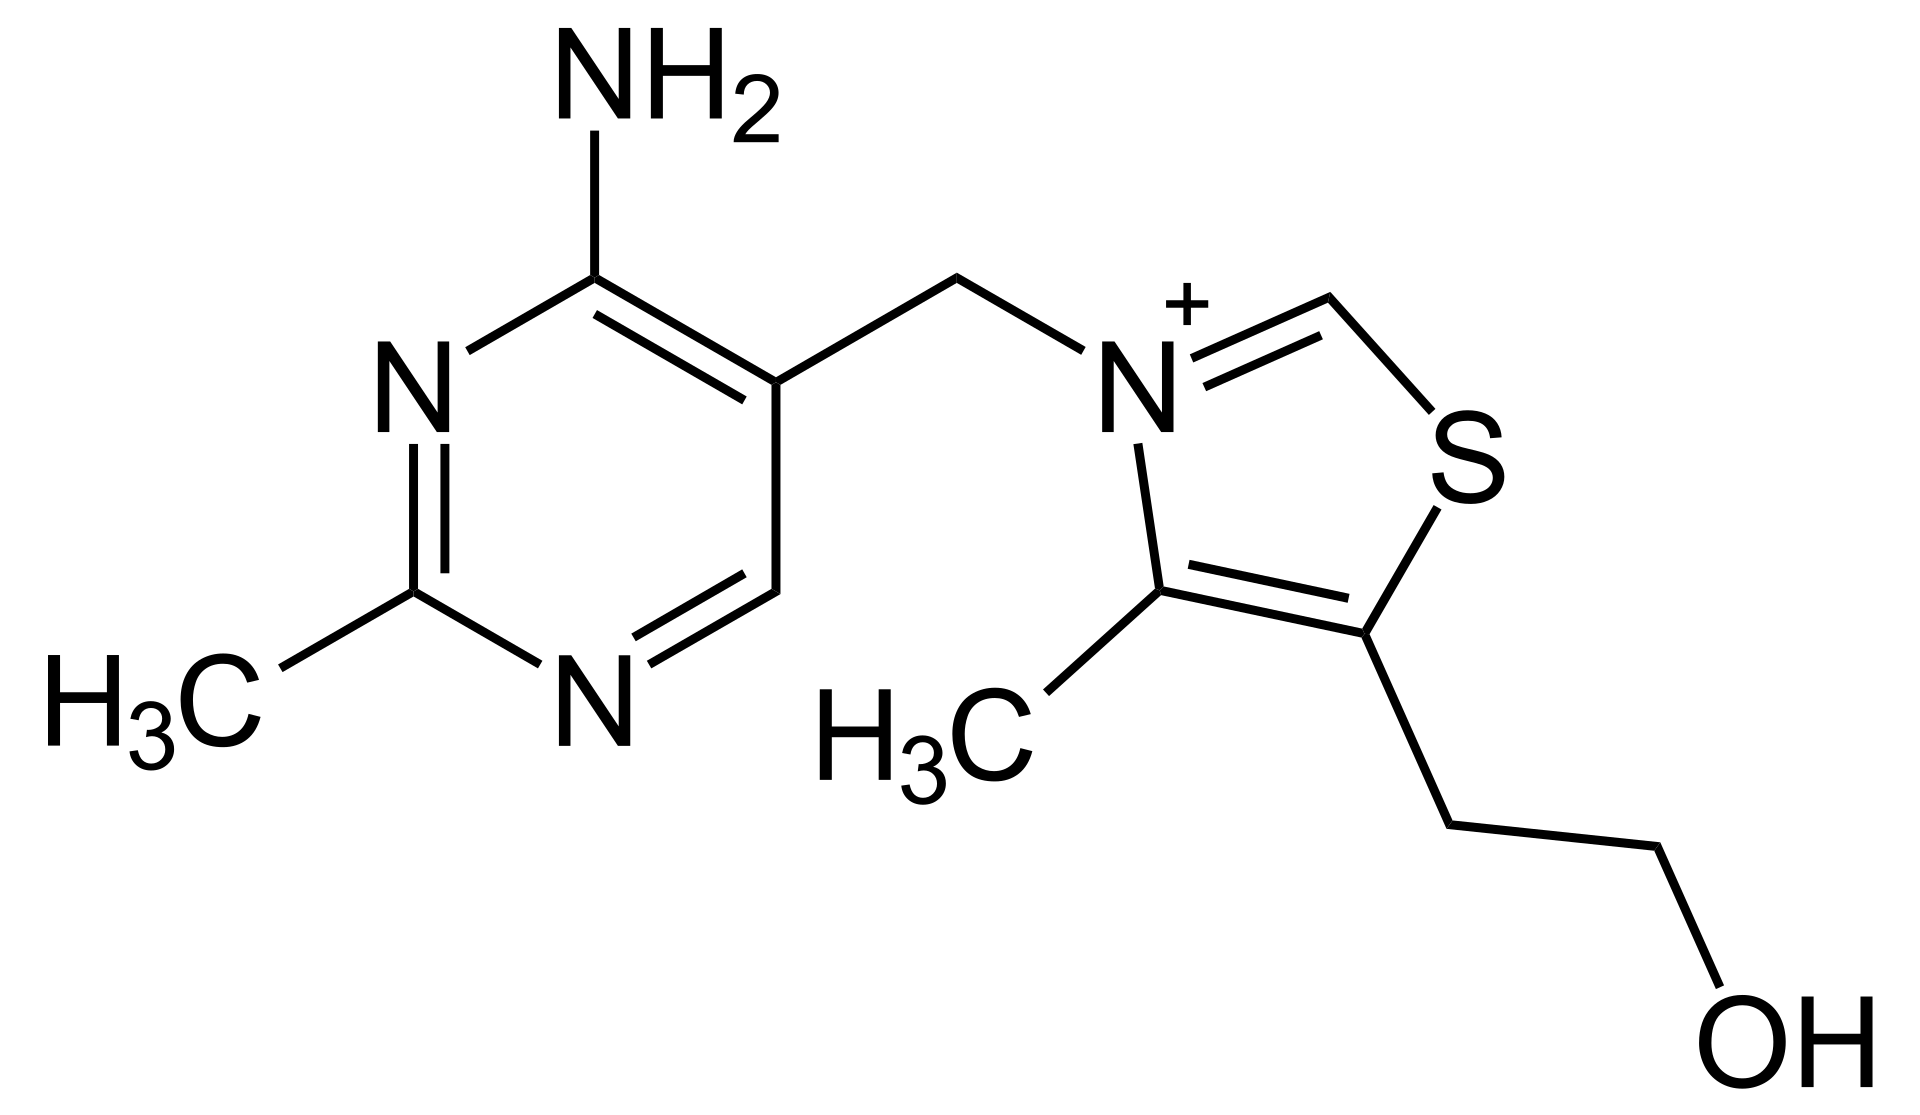
\includegraphics[width=\textwidth]{images/Vitamin_B1_chemical_structure}
\end{figure}
\newpage

\section{About}
Vitamin B\textsubscript{1}, also known as thiamine or thiamin, is an essential micronutrient that is water soluble.

It is a cation and usually it is supplied as a chloride salt. In the body the most well known and studied derivative of it is TPP (thiamine pyrophosphate), which is a coenzyme used in the catabolism of sugars and amino acids.

\section{Dietary recommendations}
Listed below are the recommendations from the US National Academy of Medicine. Data summarized from \href{https://nap.nationalacademies.org/read/6015/chapter/6}{\textit{this document}}.

The acronyms used are:
\begin{itemize}
	\item RDA --- Recommended Dietary Allowance
	\item UL --- Upper Limit
\end{itemize}

\textbf{Note}: Neither the US National Academy of Medicine nor the European Food Safety Authority have determined the tolerable upper intake level for thiamine.

\begin{table}[h]
	\caption{Thiamine Daily Reference Intakes}
	\centering \begin{tabular}{| r | c | c |}
		\hline
		\textbf{Life stage group} & \textbf{RDA} & \textbf{UL}\\ 
		& \textbf{(mg/day)} & \textbf{(mg/day)}\\ \hline
		Infants (0--6 months) & 0.2 & unknown\\ \hline
		Infants (7--12 months) & 0.3 & unknown\\ \hline
		Children (1--3 years) & 0.5 & unknown\\ \hline
		Children (4--8 years) & 0.6 & unknown\\ \hline
		Children (9--13 years) & 0.9 & unknown\\ \hline
		Females (14--18 years) & 1.0 & unknown\\ \hline
		Males (\textgreater14 years) & 1.2 & unknown\\ \hline
		Females (\textgreater19 years) & 1.1 & unknown\\ \hline
		Pregnant females (14--50 years) & 1.4 & unknown\\ \hline
		Lactating females (14--50 years) & 1.4 & unknown\\ \hline
	\end{tabular}
\end{table}
\newpage

\section{Sources}


\chapter{Vitamin B\textsubscript{2}}
\begin{figure}[h]
	\caption{Chemical structure of riboflavin}
	\centering 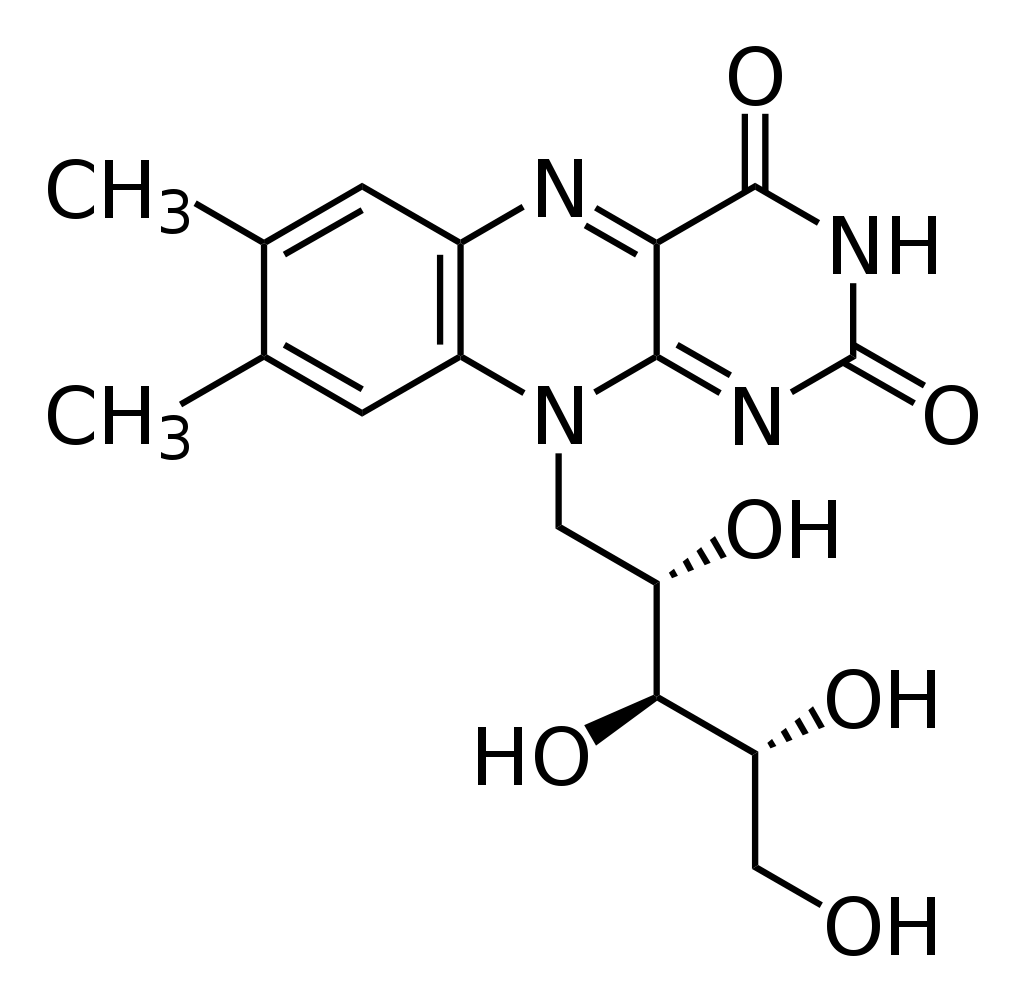
\includegraphics[width=\textwidth]{images/Vitamin_B2_chemical_structure}
\end{figure}
\newpage

\section{About}
Vitamin B\textsubscript{2}, also known as riboflavin, is an essential micronutrient that is water soluble. It is needed in the synthesis of two major coenzymes: FMN (flavin mononucleotide) and FAD (flavin adenine dinucleotide). These coenzymes are involved in energy metabolism, cellular respiration, and antibody production, as well as normal growth and development.

\section{Dietary recommendations}
Listed below are the recommendations from the US National Academy of Medicine. Data summarized from \href{https://nap.nationalacademies.org/read/6015/chapter/7}{\textit{this document}}.

The acronyms used are:
\begin{itemize}
	\item RDA --- Recommended Dietary Allowance
	\item AI --- Adequate Intake
	\item UL --- Upper Limit
\end{itemize}

\textbf{Note}: Since riboflavin is water soluble, the excess will either not be absorbed or, if absorbed, will be excreted via the kidneys into urine, resulting in a bright yellow colour known as flavinuria. There have been no documented adverse effects from taking too much vitamin B\textsubscript{2}.

\begin{table}[h]
	\caption{Riboflavin Daily Reference Intakes}
	\centering \begin{tabular}{| r | c | c |}
		\hline
		\textbf{Life stage group} & \textbf{RDA or AI(*)} & \textbf{UL}\\
		& \textbf{(mg/day)} & \textbf{(mg/day)}\\ \hline
		Infants (0--6 months) & 0.3* & unknown\\ \hline
		Infants (7--12 months) & 0.4* & unknown\\ \hline
		Children (1--3 years) & 0.5 & unknown\\ \hline
		Children (4--8 years) & 0.6 & unknown\\ \hline
		Children (9--13 years) & 0.9 & unknown\\ \hline
		Females (14--18 years) & 1.0 & unknown\\ \hline
		Males (14--18 years) & 1.3 & unknown\\ \hline
		Females (\textgreater19 years) & 1.1 & unknown\\ \hline
		Males (\textgreater19 years) & 1.3 & unknown\\ \hline
		Pregnant females (14--50 years) & 1.4 & unknown\\ \hline
		Lactating females (14--50 years) & 1.6 & unknown\\ \hline
	\end{tabular}
\end{table}
\newpage

\section{Sources}


\chapter{Vitamin B\textsubscript{3}}
\begin{figure}[h]
	\caption{Chemical structure of niacin}
	\centering 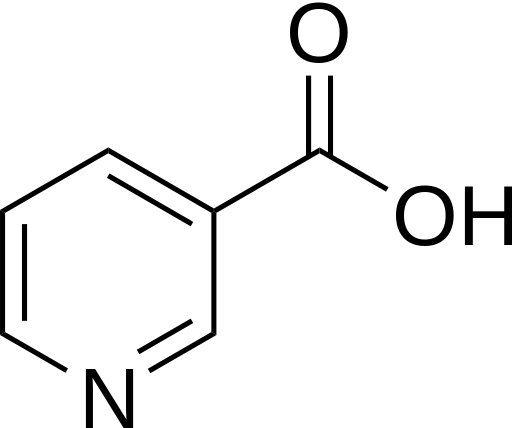
\includegraphics[width=0.49\textwidth]{images/Vitamin_B3_chemical_structure_niacin}
\end{figure}
\begin{figure}[h]
	\caption{Chemical structure of nicotinamide}
	\centering 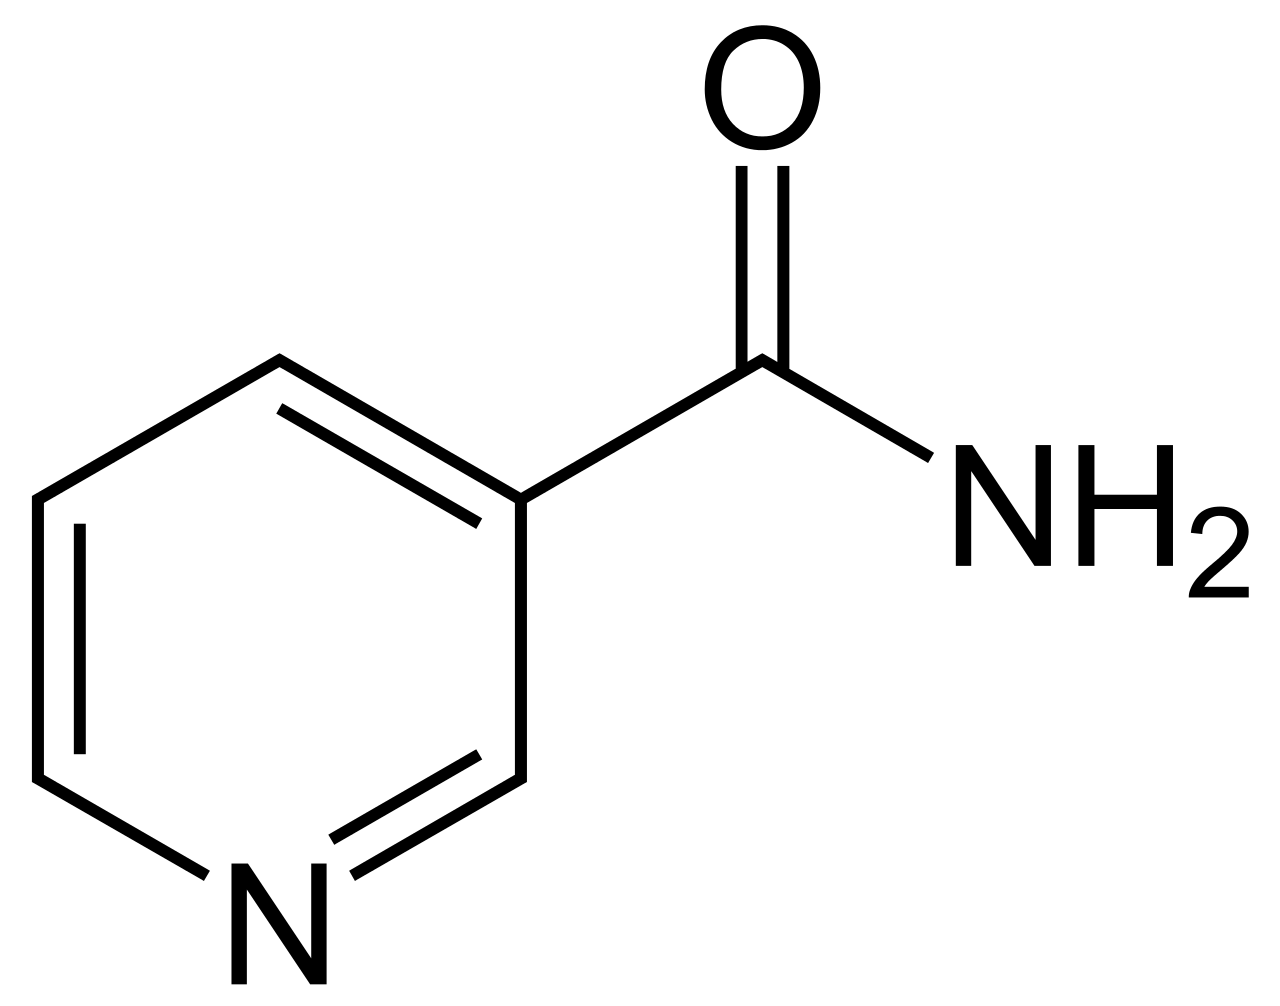
\includegraphics[width=0.56\textwidth]{images/Vitamin_B3_chemical_structure_nicotinamide}
\end{figure}
\newpage

\section{About}
Vitamin B\textsubscript{3}, colloquially referred to as niacin, is a vitamin family that includes three forms, or vitamers: niacin (nicotinic acid), nicotinamide (niacinamide), and nicotinamide riboside.

All three forms of vitamin B\textsubscript{3} are converted within the body to NAD (Nicotinamide Adenine Dinucleotide). NAD is an essential molecule that can only be made within the human body from vitamin B\textsubscript{3} or tryptophan.

\section{Dietary recommendations}
Listed below are the recommendations from the US National Academy of Medicine. Data summarized from \href{https://nap.nationalacademies.org/read/6015/chapter/8}{\textit{this document}}.

The acronyms used are:
\begin{itemize}
	\item RDA --- Recommended Dietary Allowance
	\item AI --- Adequate Intake
	\item UL --- Upper Limit
\end{itemize}

\textbf{Note}: Since tryptophan can also be used to synthesize vitamin B\textsubscript{3}, a niacin equivalent has been defined. 1 mg NE is equal to 1 mg of niacin or 60 mg of tryptophan.

\begin{table}[h]
	\caption{Niacin Daily Reference Intakes}
	\centering \begin{tabular}{| r | c | c |}
		\hline
		\textbf{Life stage group} & \textbf{RDA or AI(*)} & \textbf{UL}\\
		& \textbf{(mg NE/day)} & \textbf{(mg NE/day)}\\ \hline
		Infants (0--6 months) & 2* & unknown\\ \hline
		Infants (7--12 months) & 4* & unknown\\ \hline
		Children (1--3 years) & 6 & 10\\ \hline
		Children (4--8 years) & 8 & 15\\ \hline
		Children (9--13 years) & 12 & 20\\ \hline
		Females (14--18 years) & 14 & 30\\ \hline
		Males (14--18 years) & 16 & 30\\ \hline
		Females (\textgreater19 years) & 14 & 35\\ \hline
		Males (\textgreater19 years) & 16 & 35\\ \hline
		Pregnant females (14--18 years) & 18 & 30\\ \hline
		Pregnant females (19--50 years) & 18 & 35\\ \hline
		Lactating females (14--18 years) & 17 & 30\\ \hline
		Lactating females (19--50 years) & 17 & 35\\ \hline
	\end{tabular}
\end{table}
\newpage

\section{Sources}


\chapter{Vitamin B\textsubscript{5}}
\begin{figure}[h]
	\caption{Chemical structure of pantothenic acid}
	\centering 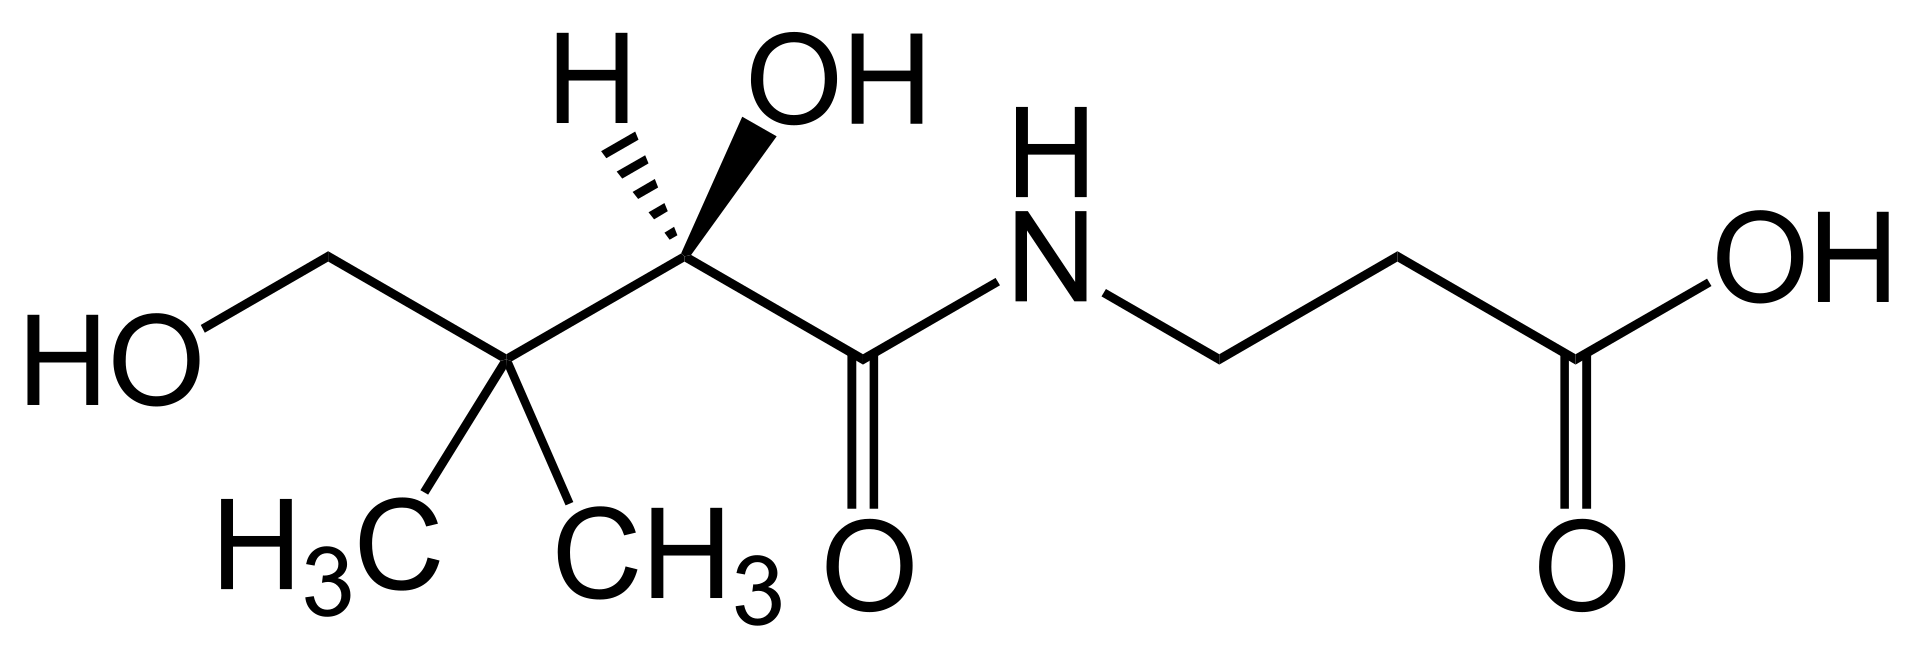
\includegraphics[width=\textwidth]{images/Vitamin_B5_chemical_structure}
\end{figure}
\newpage

\section{About}
VItamin B\textsubscript{5}, also known as pantothenic acid, is a water-soluble essential nutrient.

Pantothenic acid results from the combination of pantoic acid and \textbeta-alanine. Its name comes from Greek and it roughly translates to "from everywhere", as it can be found in almost all foods at least in small amounts. Thus, pantothenic acid deficiency is very rare in humans.

\section{Dietary recommendations}
Listed below are the recommendations from the US National Academy of Medicine. Data summarized from \href{https://nap.nationalacademies.org/read/6015/chapter/12}{\textit{this document}}.

The acronyms used are:
\begin{itemize}
	\item AI --- Adequate Intake
	\item UL --- Upper Limit
\end{itemize}

\textbf{Note}: There is no evidence of adverse effects from high doses of pantothenic acid. Therefore, there is no spcified UL.

\begin{table}[h]
	\caption{Pantothenic Acid Daily Reference Intakes}
	\centering \begin{tabular}{| r | c | c |}
		\hline
		\textbf{Life stage group} & \textbf{AI} & \textbf{UL}\\
		& \textbf{(mg/day)} & \textbf{(mg/day)}\\ \hline
		Infants (0--6 months) & 1.7 & unknown\\ \hline
		Infants (7--12 months) & 1.8 & unknown\\ \hline
		Children (1--3 years) & 2 & unknown\\ \hline
		Children (4--8 years) & 3 & unknown\\ \hline
		Children (9--13 years) & 4 & unknown\\ \hline
		Adult men and women (\textgreater19 years) & 5 & unknown\\ \hline
		Pregnant females (14--50 years) & 6 & unknown\\ \hline
		Lactating females (14--50 years) & 7 & unknown\\ \hline
	\end{tabular}
\end{table}
\newpage

\section{Sources}


\chapter{Vitamin B\textsubscript{6}}
\begin{figure}[h]
	\caption{Chemical structure of pyridoxal 5'-phosphate (left) and pyridoxal (right)}
	\centering {
	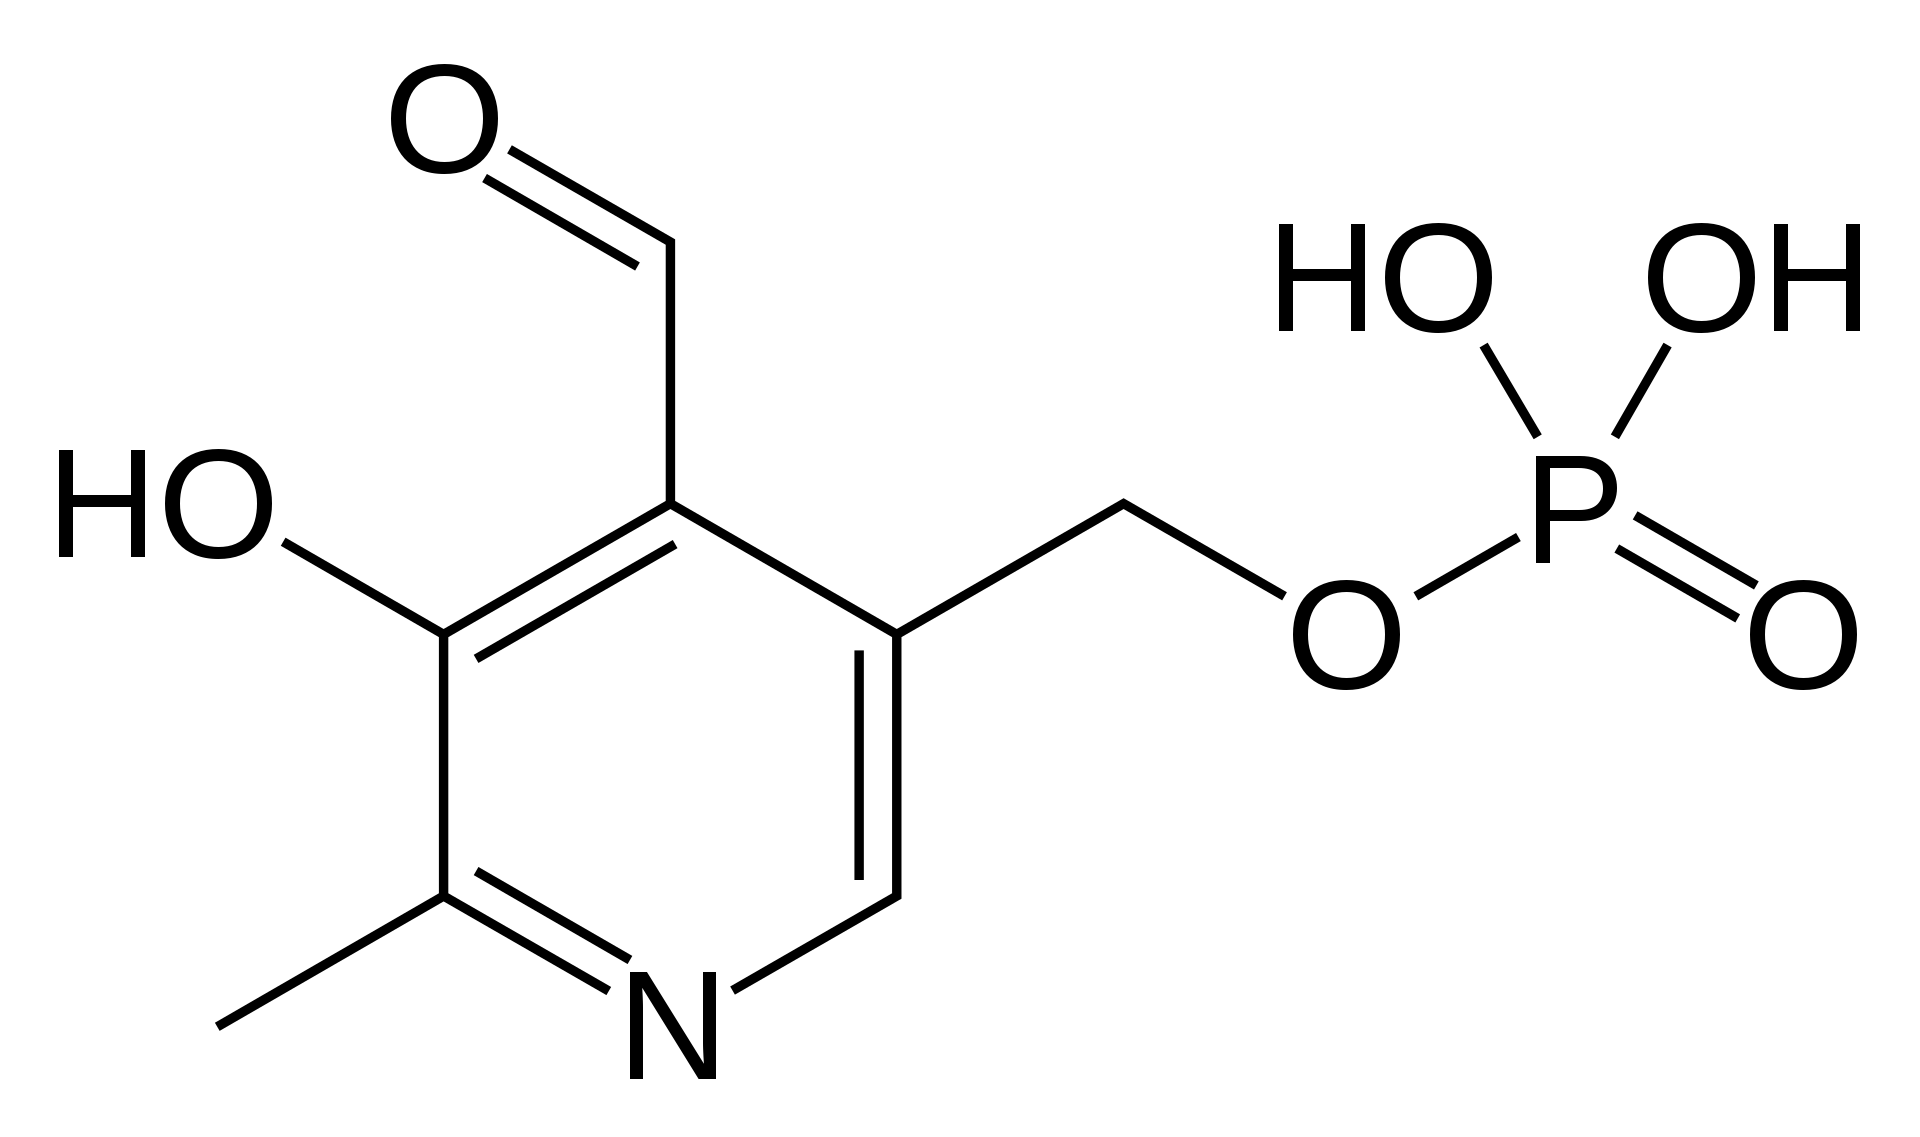
\includegraphics[width=0.4\textwidth]{images/Vitamin_B6_chemical_structure_pyridoxal_phosphate}
	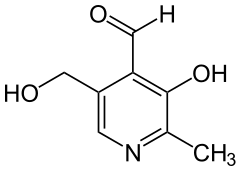
\includegraphics[width=0.33\textwidth]{images/Vitamin_B6_chemical_structure_pyridoxal}
	}
\end{figure}
\begin{figure}[h]
	\caption{Chemical structure of pyridoxine (left) and pyridoxamine (right)}
	\centering {
	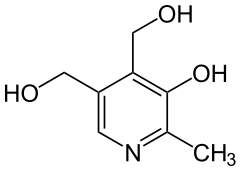
\includegraphics[width=0.33\textwidth]{images/Vitamin_B6_chemical_structure_pyridoxine}
	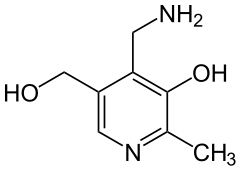
\includegraphics[width=0.33\textwidth]{images/Vitamin_B6_chemical_structure_pyridoxamine}
	}
\end{figure}
\newpage

\section{About}
Vitamin B\textsubscript{6} is an essential nutrient family of vitamers, which includes: PLP (PyridoxaL 5'-Phosphate) (the active form), PL (PyridoxaL), PNP (PyridoxiNe 5'-Phosphate), PN (PyridoxiNe), PMP (PyridoxaMine 5'-Phosphate), and PM (PyridoxaMine).

 Vitamin B\textsubscript{6} is a water-soluble vitamin. All of its vitamers get converted in the body to PLP.

 Vitamin B\textsubscript{6} serves as a co-factor in more than 140 cellular reactions, mostly related to amino acid biosynthesis and catabolism.

\section{Dietary recommendations}
Listed below are the recommendations from the US National Academy of Medicine. Data summarized from \href{https://nap.nationalacademies.org/read/6015/chapter/9}{\textit{this document}}.

The acronyms used are:
\begin{itemize}
	\item RDA --- Recommended Dietary Allowance
	\item AI --- Adequate Intake
	\item UL --- Upper Limit
\end{itemize}

\textbf{Note}: There is no evidence of adverse effects from high doses of vitamin B\textsubscript{6} from food sources.There are documented side effects (sensory neuropathy and dermatological lesions) associated with high intake of supplemental vitamin B\textsubscript{6} in the form of pyridoxine.

\begin{table}[h]
	\caption{Vitamin B\textsubscript{6} Daily Reference Intakes}
	\centering \begin{tabular}{| r | c | c |}
		\hline
		\textbf{Life stage group} & \textbf{RDA or AI(*)} & \textbf{UL (as PN)}\\
		& \textbf{(mg/day)} & \textbf{(mg/day)}\\ \hline
		Infants (0--6 months) & 0.1* & unknown\\ \hline
		Infants (7--12 months) & 0.3* & unknown\\ \hline
		Children (1--3 years) & 0.5 & 30\\ \hline
		Children (4--8 years) & 0.6 & 40\\ \hline
		Children (9--13 years) & 1.0 & 60\\ \hline
		Females (14--18 years) & 1.2 & 80\\ \hline
		Males (14--18 years) & 1.3 & 80\\ \hline
		Adults (19--50 years) & 1.3 & 100\\ \hline
		Females (\textgreater50 years) & 1.5 & 100\\ \hline
		Males (\textgreater50 years) & 1.7 & 100\\ \hline
		Pregnant females (14--18 years) & 1.9 & 80\\ \hline
		Pregnant females (19--50 years) & 1.9 & 100\\ \hline
		Lactating females (14--18 years) & 2.0 & 80\\ \hline
		Lactating females (19--50 years) & 2.0 & 100\\ \hline
	\end{tabular}
\end{table}
\newpage

\section{Sources}


\chapter{Vitamin B\textsubscript{7}}
\begin{figure}[h]
	\caption{Chemical structure of Vitamin B7}
	\centering 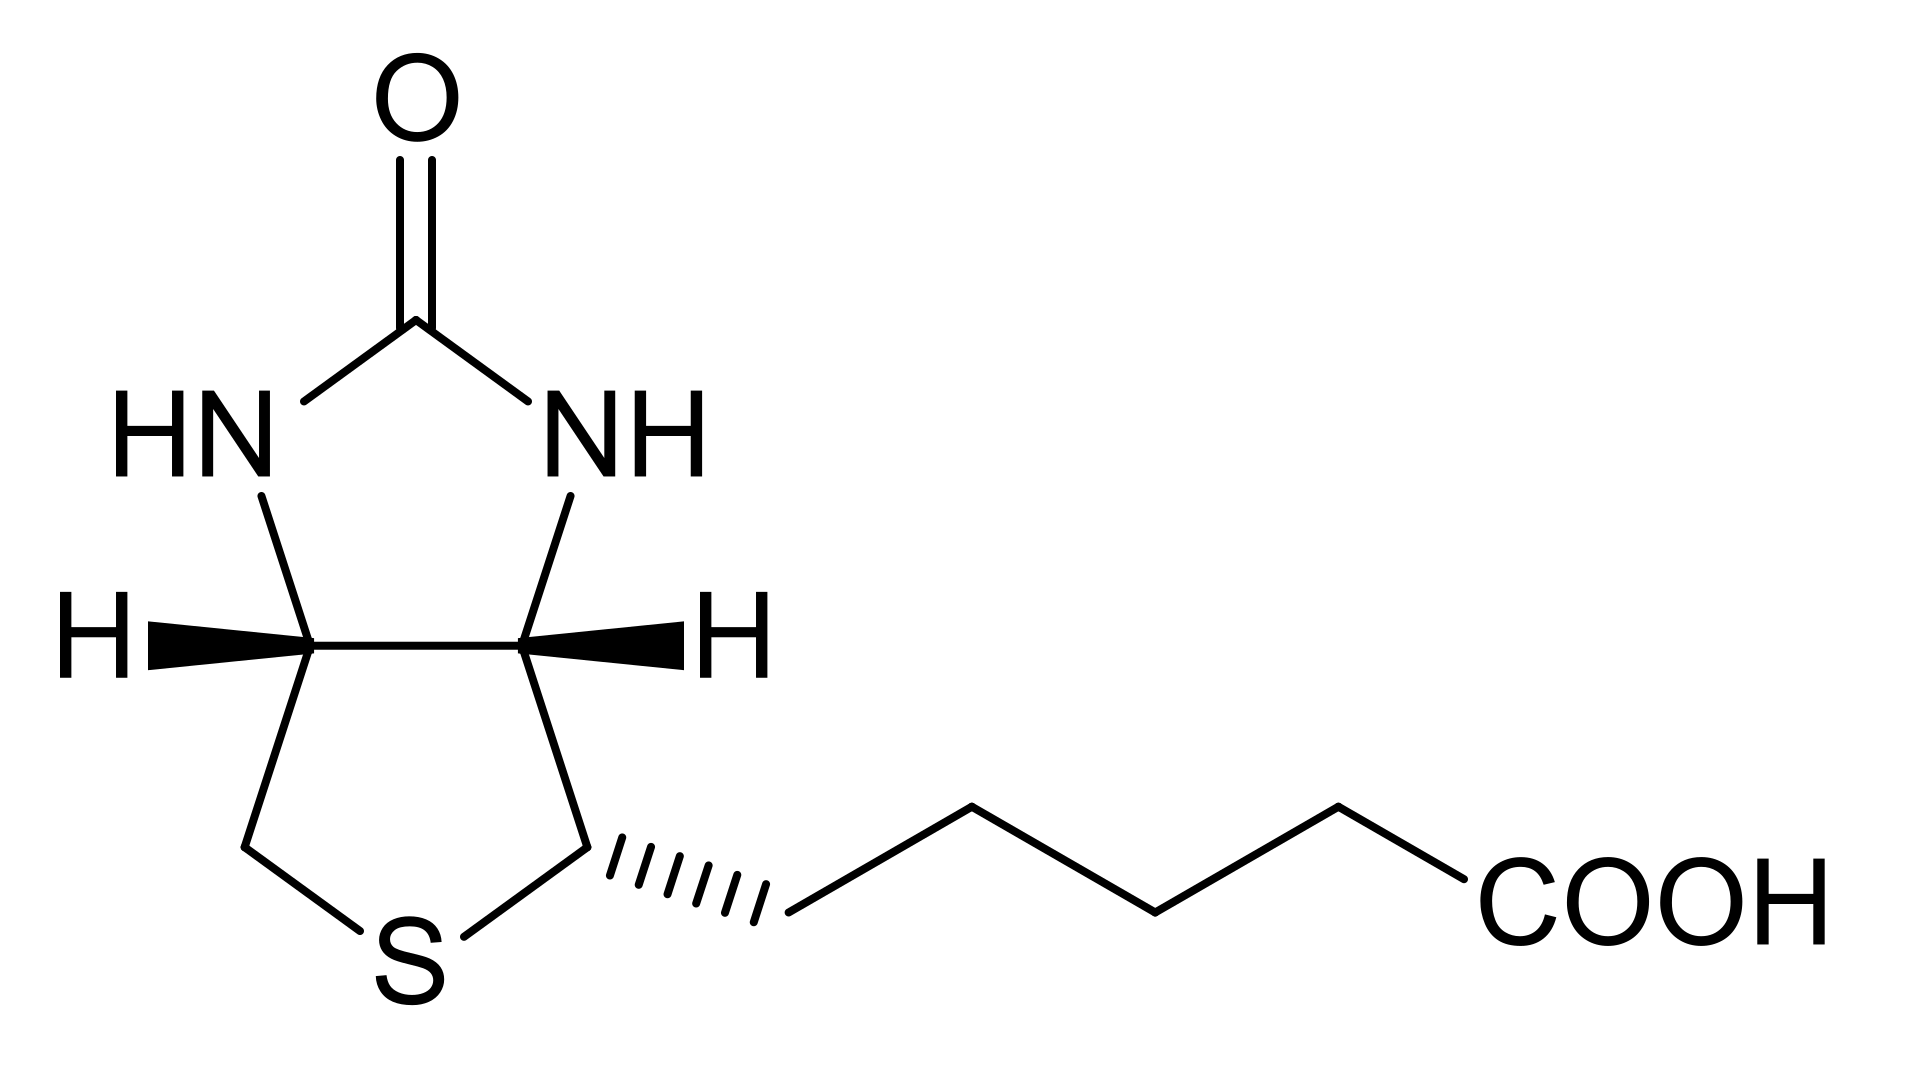
\includegraphics[width=0.75\textwidth]{images/Vitamin_B7_chemical_structure}
\end{figure}
\newpage

\section{About}


\section{Dietary recommendations}


\section{Sources}


\chapter{Vitamin B\textsubscript{9}}
\begin{figure}[h]
	\caption{Chemical structure of Vitamin B9}
	\centering 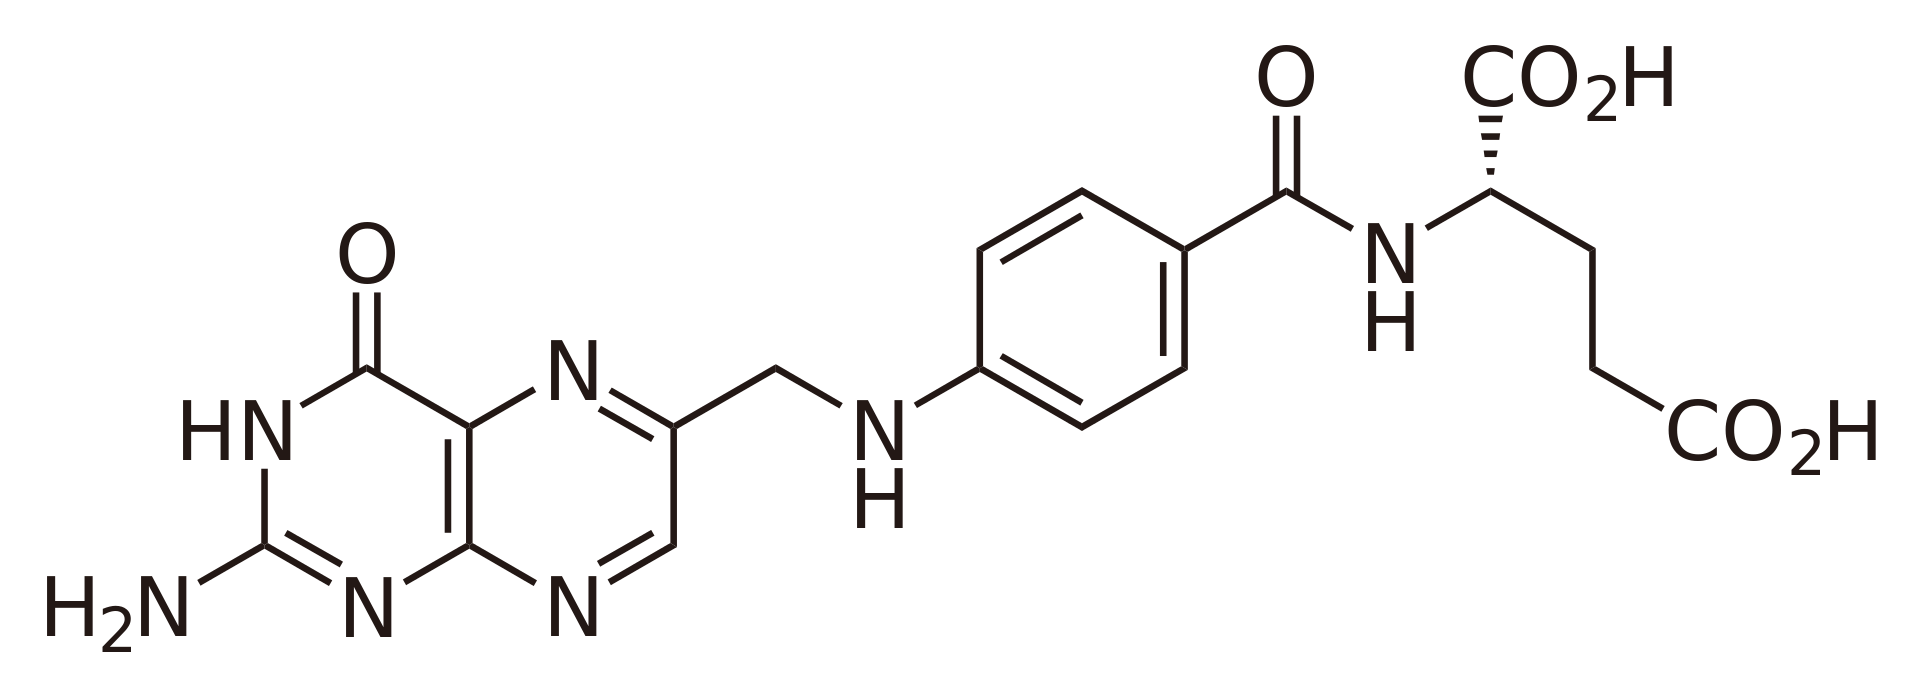
\includegraphics[width=\textwidth]{images/Vitamin_B9_chemical_structure}
\end{figure}
\newpage

\section{About}


\section{Dietary recommendations}


\section{Sources}


\chapter{Vitamin B\textsubscript{12}}
\begin{figure}[h]
	\caption{Chemical structure of Vitamin B12}
	\centering 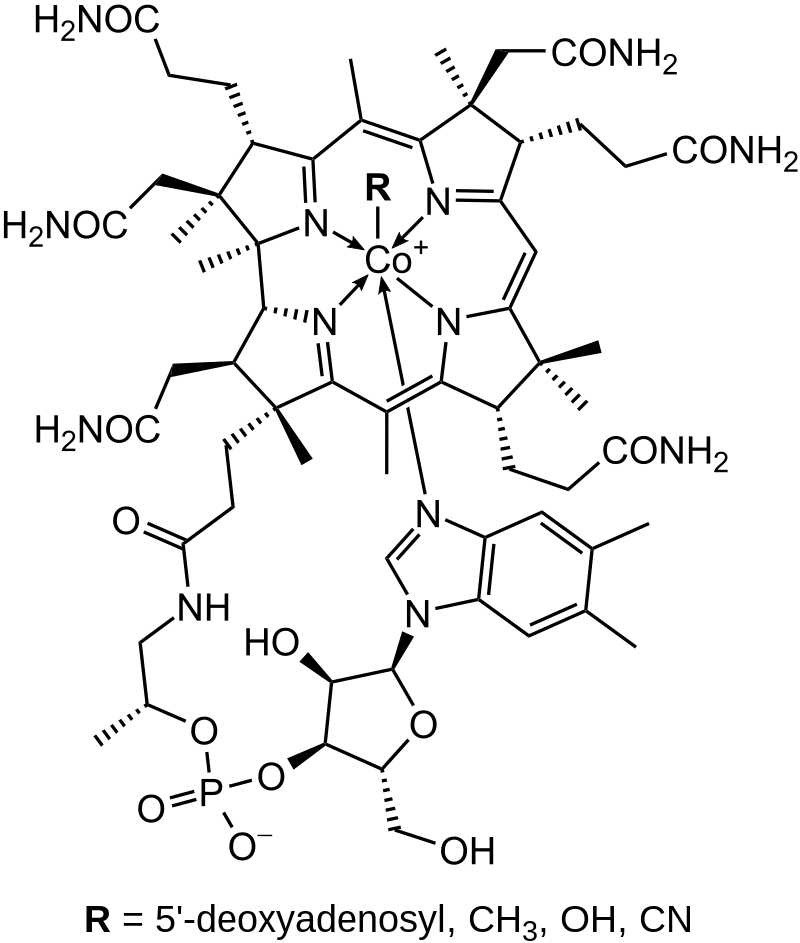
\includegraphics[width=0.5\textwidth]{images/Vitamin_B12_chemical_structure}
\end{figure}
\newpage

\section{About}


\section{Dietary recommendations}


\section{Sources}


\chapter{Vitamin C}
\begin{figure}[h]
	\caption{Chemical structure of Vitamin C}
	\centering 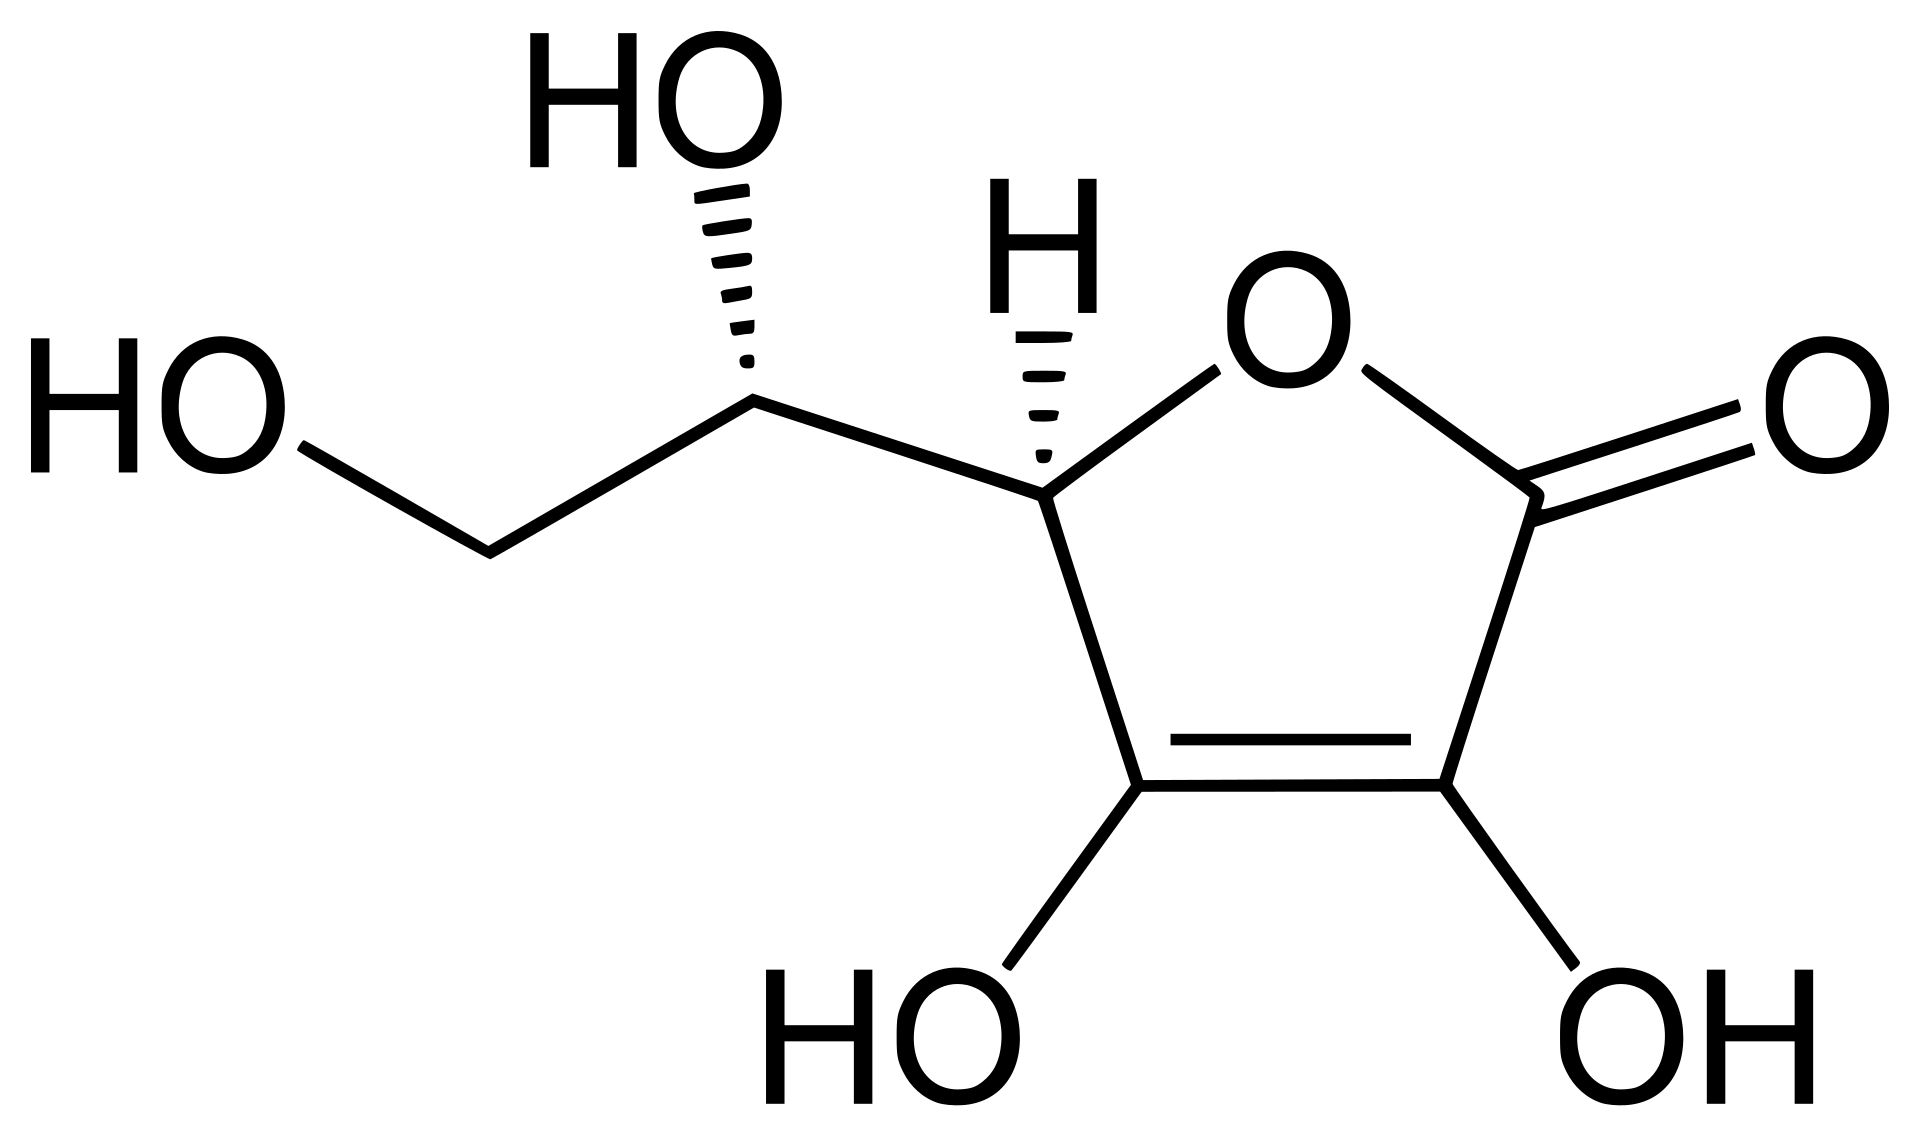
\includegraphics[width=0.75\textwidth]{images/Vitamin_C_chemical_structure}
\end{figure}
\newpage

\section{About}


\section{Dietary recommendations}


\section{Sources}


\chapter{Vitamin D}
\begin{figure}[h]
	\caption{Chemical structure of Vitamin D}
	\centering 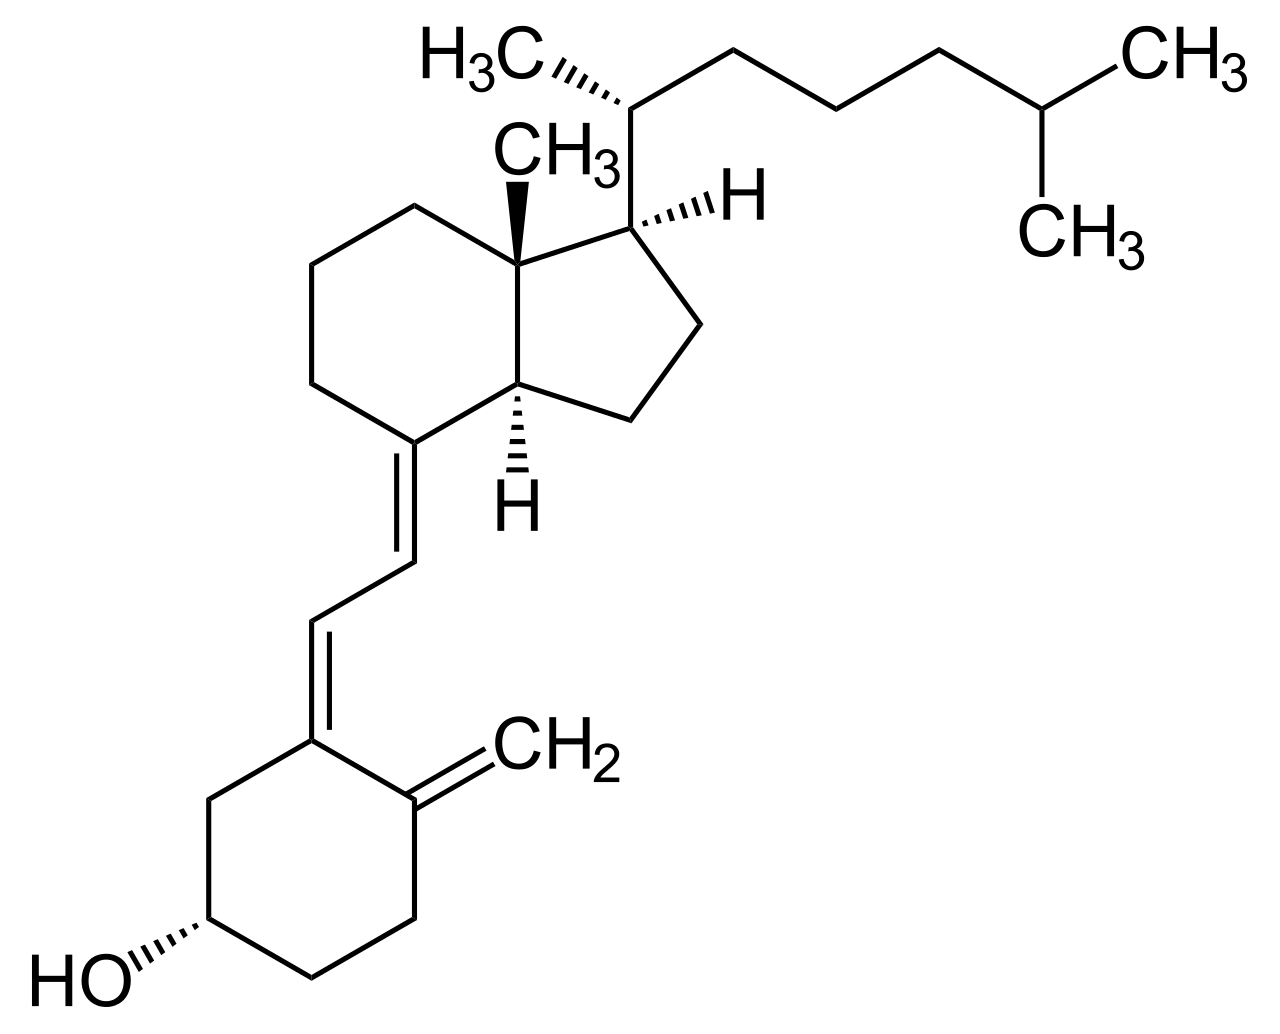
\includegraphics[width=0.75\textwidth]{images/Vitamin_D_chemical_structure}
\end{figure}
\newpage

\section{About}


\section{Dietary recommendations}


\section{Sources}


\chapter{Vitamin E}
\begin{figure}[h]
	\caption{Chemical structure of Vitamin E}
	\centering 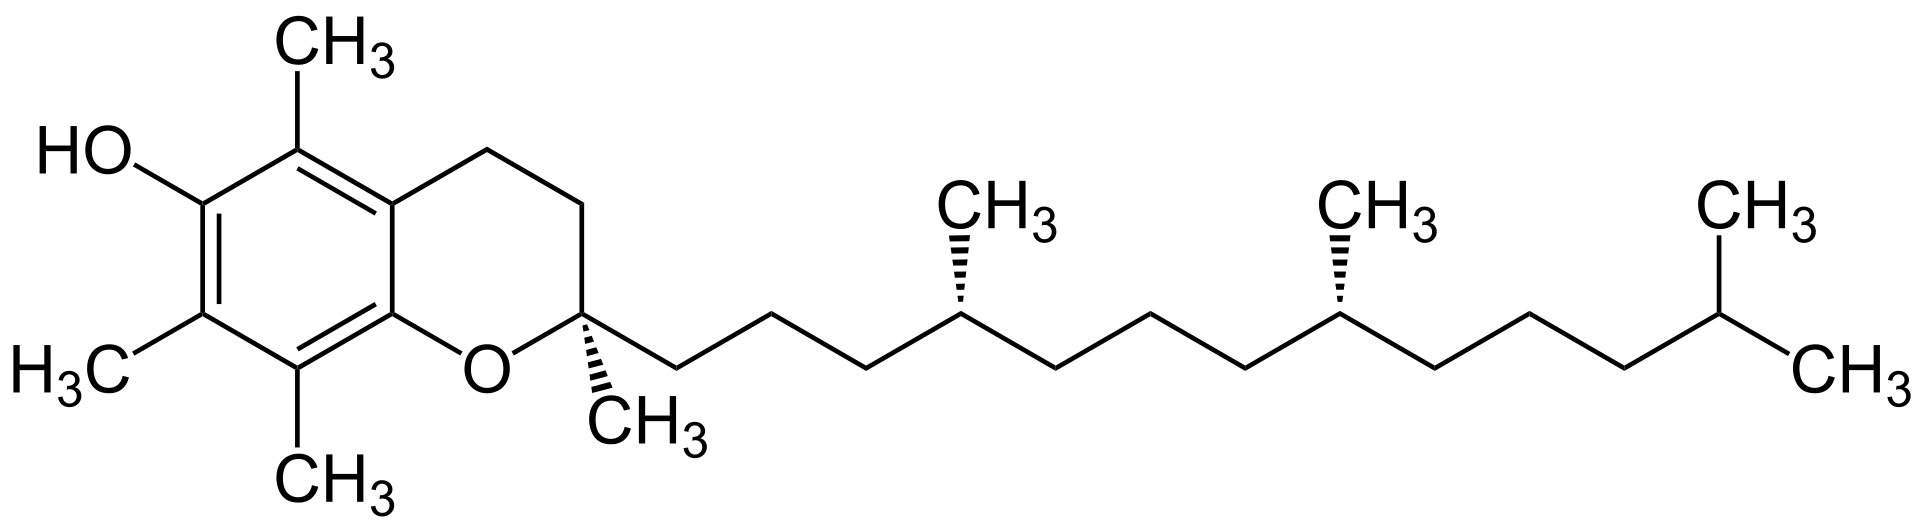
\includegraphics[width=\textwidth]{images/Vitamin_E_chemical_structure}
\end{figure}
\newpage

\section{About}


\section{Dietary recommendations}


\section{Sources}


\chapter{Vitamin K\textsubscript{1}}
\begin{figure}[h]
	\caption{Chemical structure of Vitamin K1}
	\centering 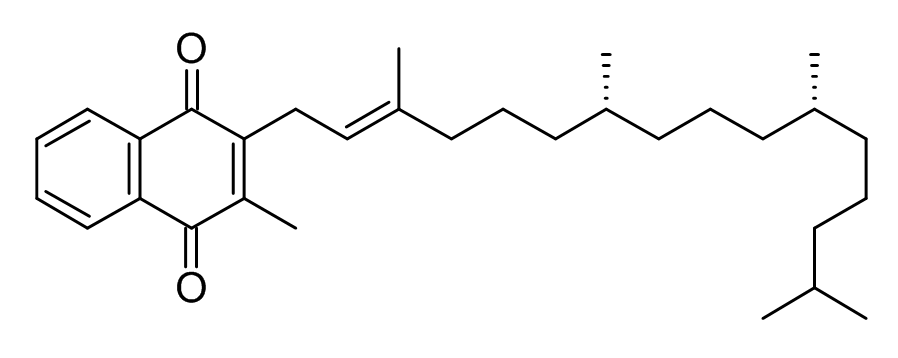
\includegraphics[width=\textwidth]{images/Vitamin_K1_chemical_structure}
\end{figure}
\newpage

\section{About}


\section{Dietary recommendations}


\section{Sources}


\chapter{Vitamin K\textsubscript{2}}
\begin{figure}[h]
	\caption{Chemical structure of Vitamin K2}
	\centering 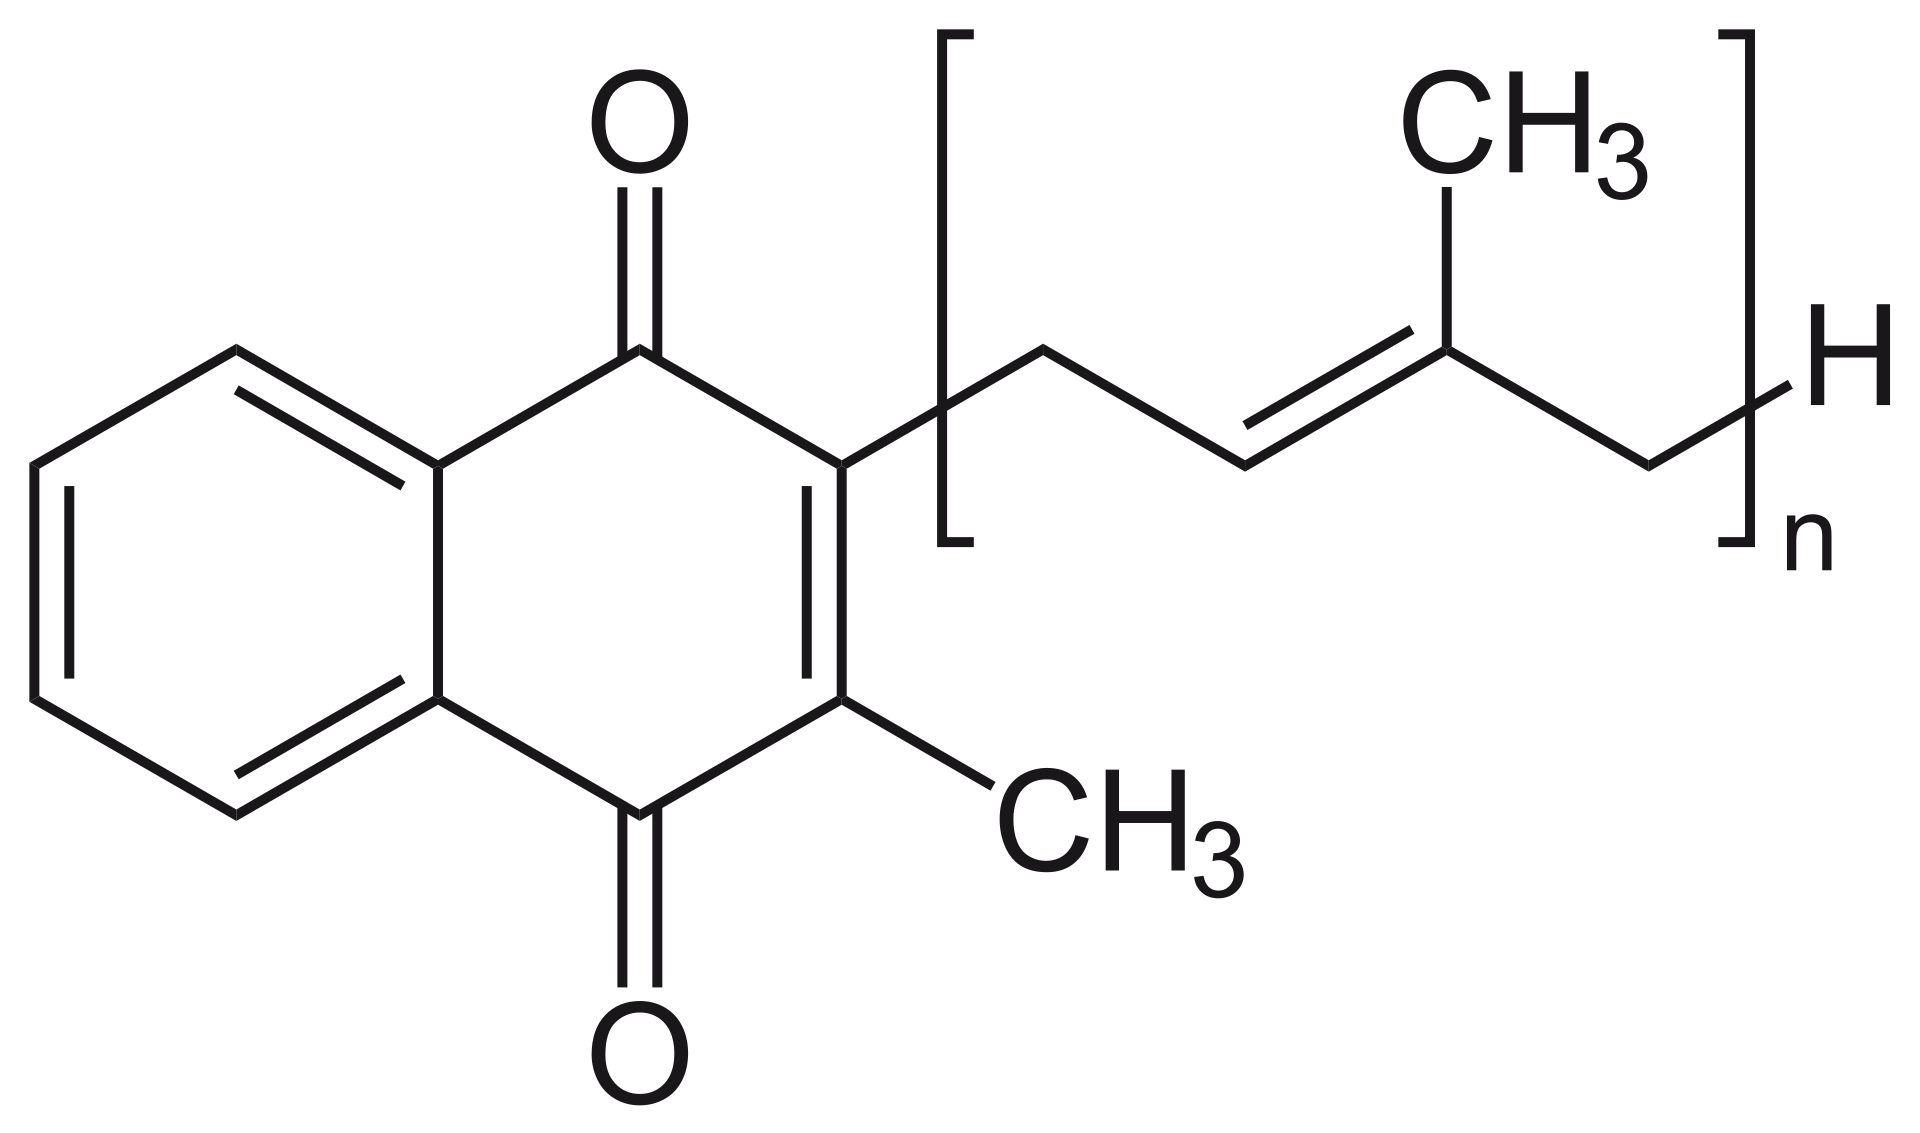
\includegraphics[width=0.75\textwidth]{images/Vitamin_K2_chemical_structure}
\end{figure}
\newpage

\section{About}


\section{Dietary recommendations}


\section{Sources}


\chapter{Vitamin K\textsubscript{3}}
\begin{figure}[h]
	\caption{Chemical structure of Vitamin K3}
	\centering 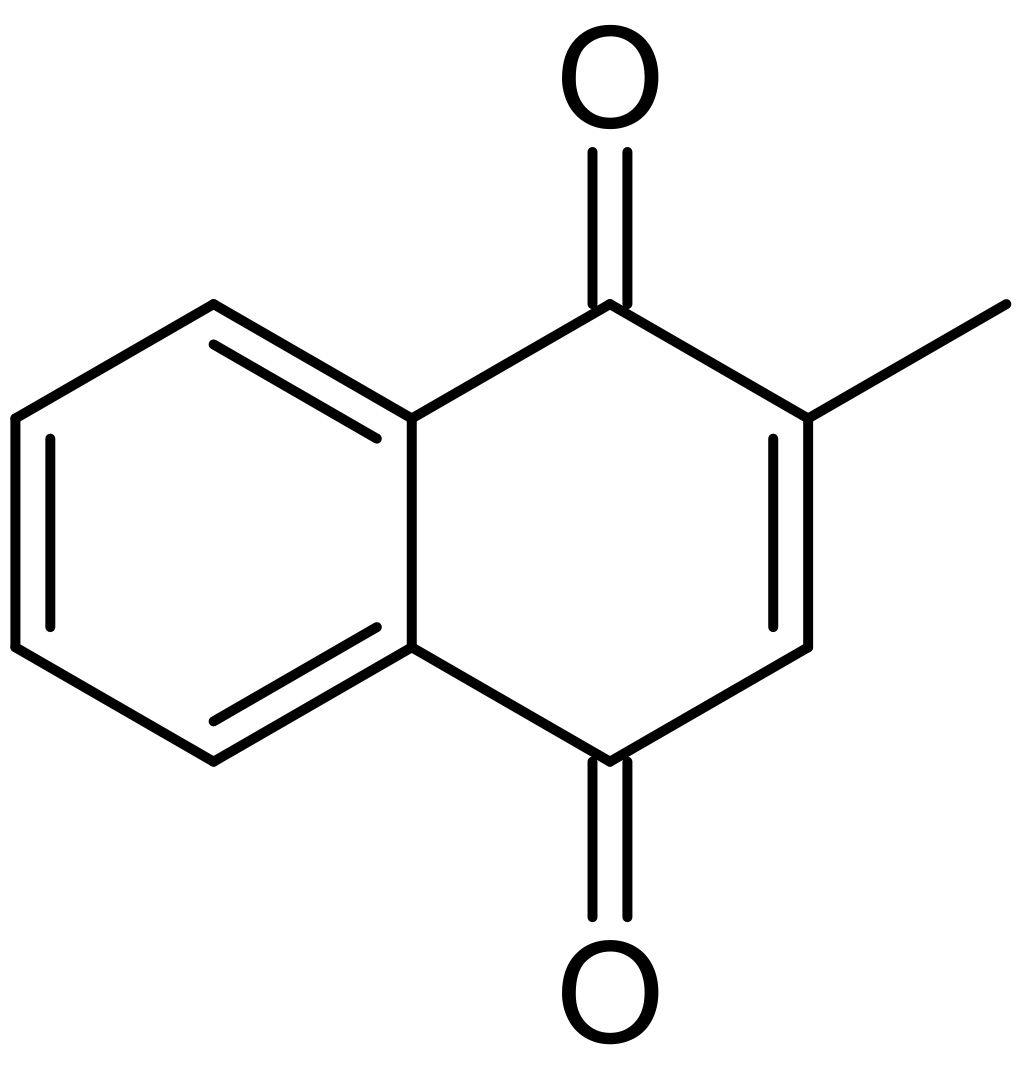
\includegraphics[width=0.5\textwidth]{images/Vitamin_K3_chemical_structure}
\end{figure}
\newpage

\section{About}


\section{Dietary recommendations}


\section{Sources}


\chapter{Choline}
\begin{figure}[h]
	\caption{Chemical structure of Choline}
	\centering 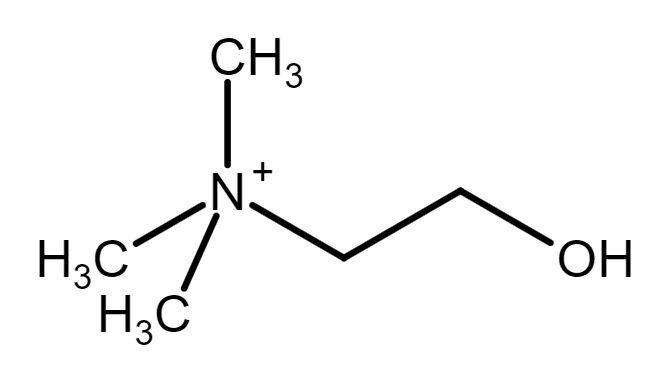
\includegraphics[width=0.75\textwidth]{images/Choline_chemical_structure}
\end{figure}
\newpage

\section{About}


\section{Dietary recommendations}


\section{Sources}


\listoffigures


\listoftables


\end{document}